\subsection{BP 8a:
Old  3D landslide (Laboratory)}

There are plans to replace this benchmark problem with a new one.
This has not yet happened.
This old benchmark problem consists of a wedge sliding on a plane beach.
See \Fig{bp8pcolor1}.


\subsubsection{Problem specification}

\begin{itemize}

\item PMEL-135, pp 7 \& 47-48 \cite{SynolakisBernard:pmel135}.

\item The original experiment is fully described on NOAA's benchmarking website which can be found at 

\url{http://nctr.pmel.noaa.gov/benchmark/Laboratory/Laboratory\_Landslide/index.html}

%\cite{NOAAbenchmark:3dlandslide}.

\end{itemize}

\begin{figure}[ht]
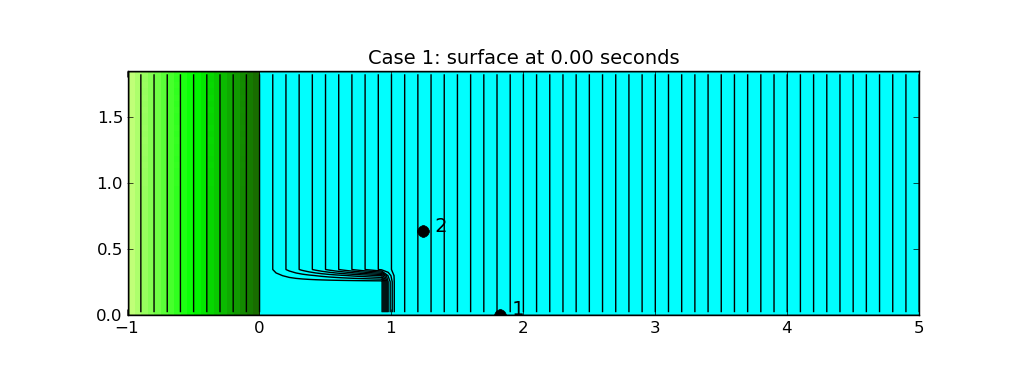
\includegraphics[width=5 in]{bp8a/frame0.png}
\vskip 10pt
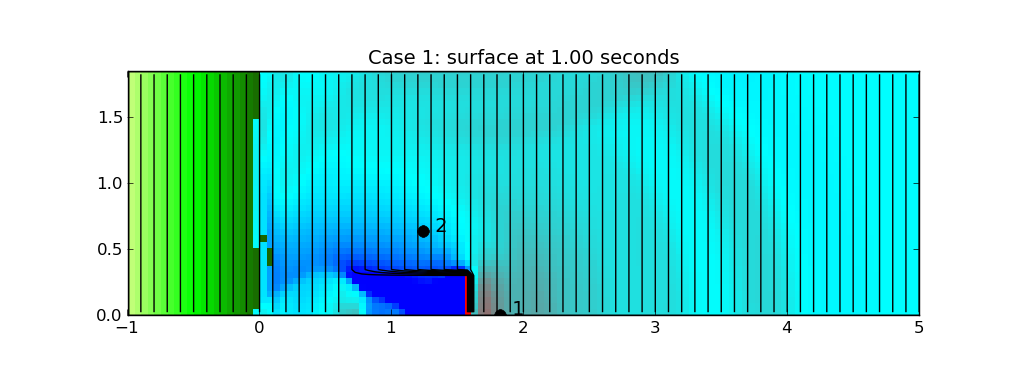
\includegraphics[width=5 in]{bp8a/frame2.png}
\vskip 10pt
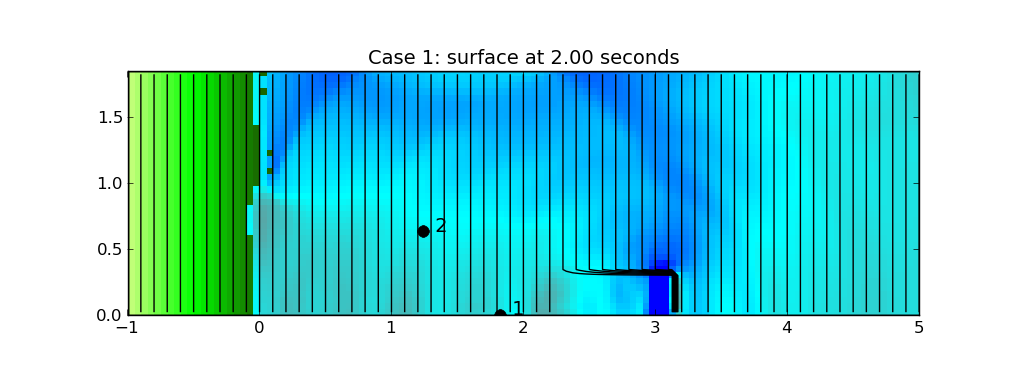
\includegraphics[width=5 in]{bp8a/frame4.png}
\caption{\label{fig:bp8pcolor1}
Single grid $140\times 40$ GeoClaw simulation of Case 1 
to illustrate moving bathymetry and gauge locations.
%Problem set up (top view).  Note that the black lines represent regions of 
%AMR refinement with the innermost region being level 3 and the outermost
%region being level 1.
  }
\end{figure}


\subsubsection{What we did}

\begin{itemize}
\item We solved the nonlinear shallow water equations in Cartesian
coordinates with $g=9.81$ and no friction.

\item We used the given laboratory data and problem set up to create our
initial topography and bathymetry.  While there was data provided up to
time 20 s, we only conducted simulations up to time 10 s, as was done on 
NOAA's benchmarking website.  We specified the movement of the wedge
by using the time histories of the block motion provided for the problem.  
In order to implement this, we adjusted the bathymetry every time step to
capture the wedge sliding down the linear beach.  The slope of this linear
beach was $\frac{1}{2}$.  Due to the symmetry of the problem, we simplified the
problem to half of the domain of the tank, specifying an outflow or non-reflecting
boundary condition at the right boundary so reflected waves exit.  We also
specified a solid wall boundary condition at all other boundaries.
(Note that the wave tank was much longer than computational domain specified.)
Zero-order extrapolation,
which generally gives a very good approximation to non-reflecting boundary
conditions as described in Section 7.3.1 of \cite{rjl:fvmhp}.  Solid wall
boundary conditions are implemented as described in Section 7.3.3 of
\cite{rjl:fvmhp}.

%\item See \Fig{bp8pcolor1} for a better picture of the problem set up.

\item  The moving bathymetry is handled by recomputing $B_{ij}^n =
B(x_i,y_j,t_n)$ in
each time step, at the center of each finite volume grid cell, based on the
specified bathymetry.
This is the standard approach
for handling moving bathymetry in GeoClaw:  the value $B_{ij}^n$ is adjusted
but the fluid depth $h_{ij}^n$ remains the same, so that the water column is
simply displaced vertically in any cell where the bathymetry changes.  For
bathymetry that is smoothly varying  in space and time
this is considered a reasonable approach.  Note, however, that no momentum
is directly imparted to the water by the moving bathymetry.  

For this problem, the vertical face of the wedge makes this approach
inadequate.  The discontinuity in the moving bathymetry means that in each
time step the bathymetry near the face will gain a increment of 0.455 m,
lifting the water in this cell by this amount.  This is not at all physical.
Instead, the moving face should impart horizontal momentum to the water.

Given this inaccuracy and the full three-dimensional nature of the physical
flow, we do not expect to obtain very good comparisons computationionally.

\item We solved on $35\times 10$ grid with 3 levels of adaptive mesh refinement.
We refined in the $x$- and $y$- directions by a factor of 6 from levels 1 to 2 and
levels 2 to 3.  We refined in time by a factor of 3.  We specified level 3 refinement
on a rectangle with $x$ values of $[-0.4, 2]$ and $y$ values of $[0, 1]$.

\item We compared the simulated gauge data with the laboratory gauge data 
to determine GeoClaw's accuracy on this problem.
\end{itemize}

\ignore{
\subsubsection{Simulations}

See \Fig{bp8pcolorcase1} for frames of the Case 1 simulation in GeoClaw, and
\Fig{bp8pcolorcase2} for frames of the Case 2 simulation.
Note that
these only go up to time 1.2 seconds.

\begin{figure}[ht]
\hfil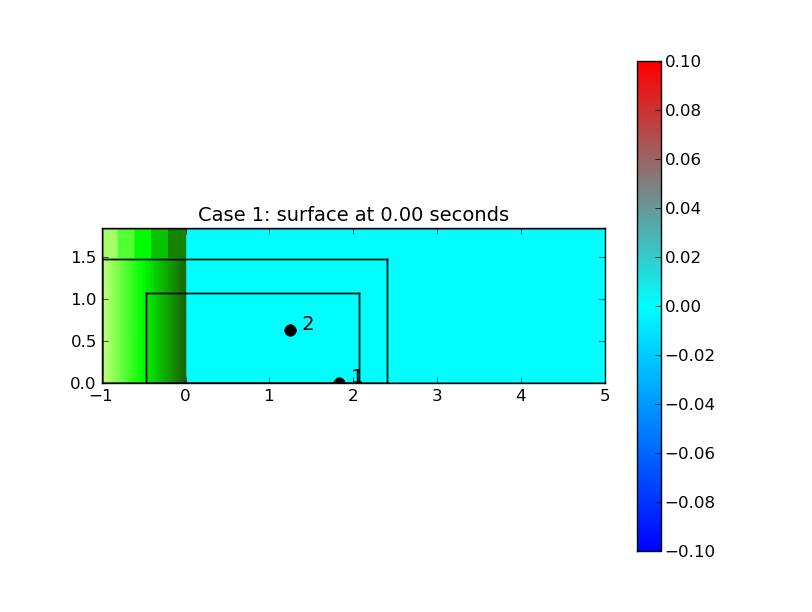
\includegraphics[width=2.8in]{bp12/case1pcolor0.png}\hfil
\hfil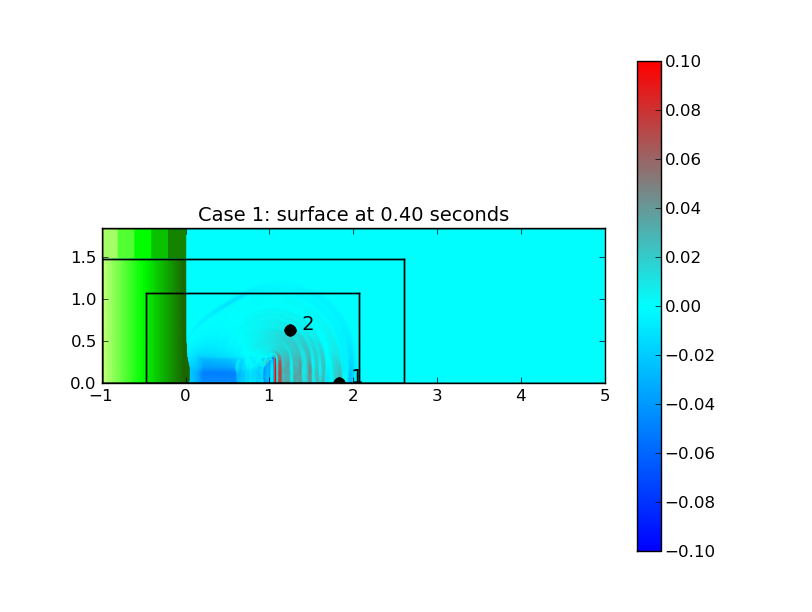
\includegraphics[width=2.8in]{bp12/case1pcolor4.png}\hfil
\vskip 5pt
\hfil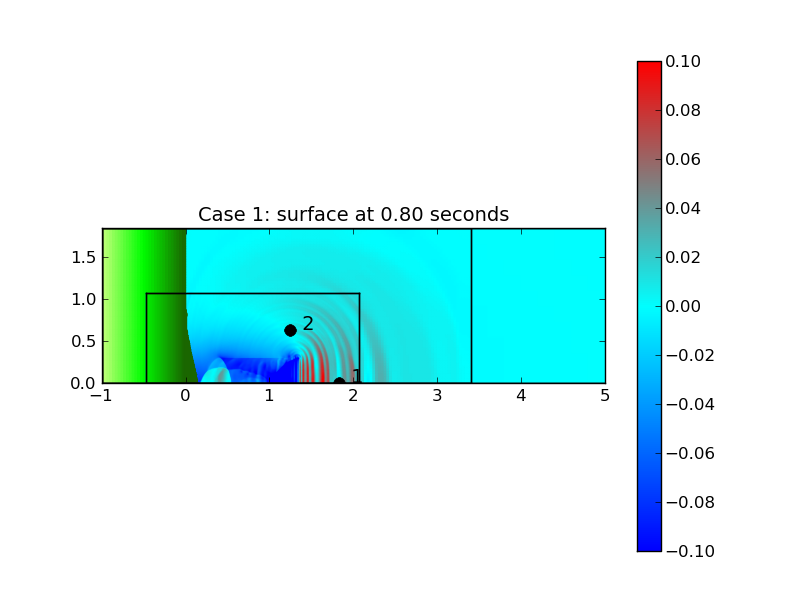
\includegraphics[width=2.8in]{bp12/case1pcolor8.png}\hfil
\hfil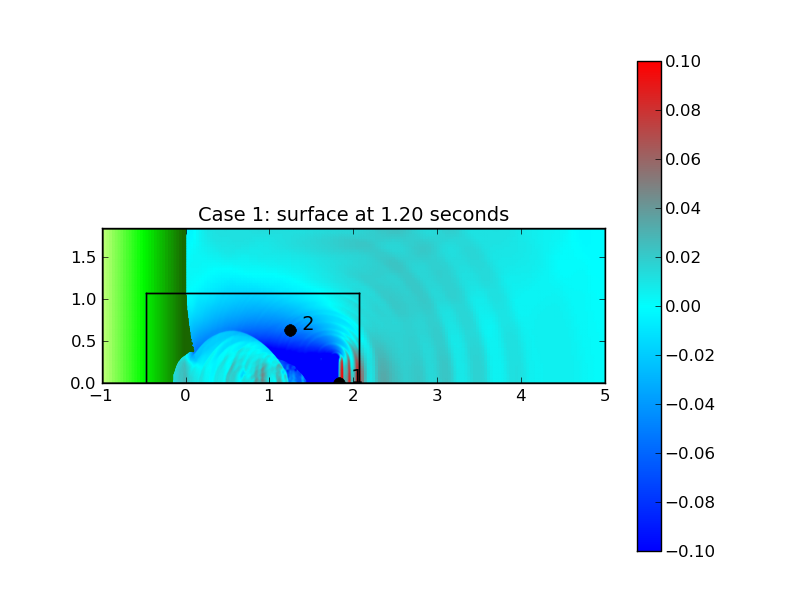
\includegraphics[width=2.8in]{bp12/case1pcolor12.png}\hfil
\caption{\label{fig:bp8pcolorcase1}
GeoClaw simulation for case 1 at times $t = 0,$ 0.4, 0.8, and 1.2.
  }
\end{figure}


\begin{figure}[ht]
\hfil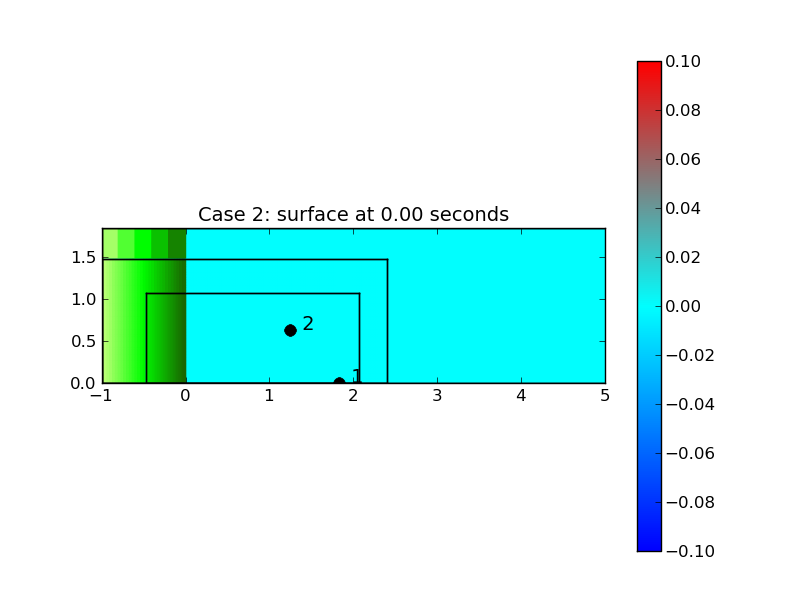
\includegraphics[width=2.8in]{bp12/case2pcolor0.png}\hfil
\hfil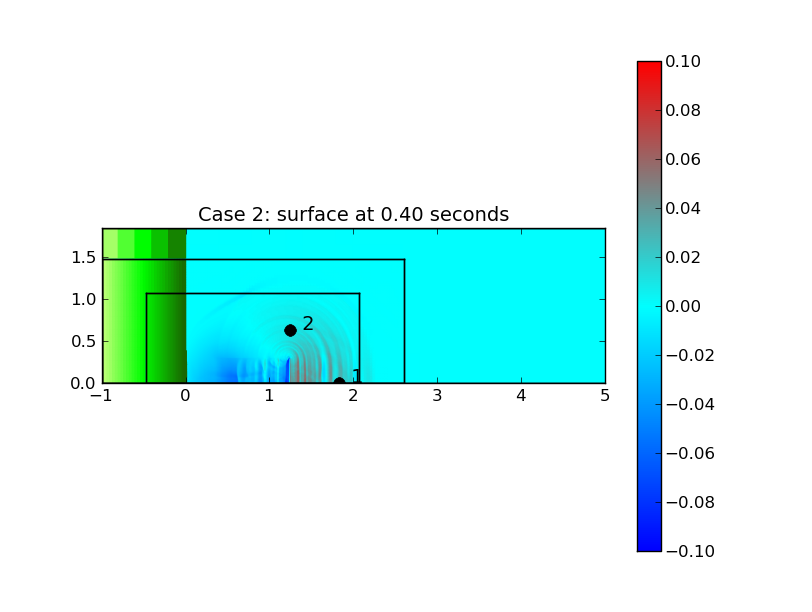
\includegraphics[width=2.8in]{bp12/case2pcolor4.png}\hfil
\vskip 5pt
\hfil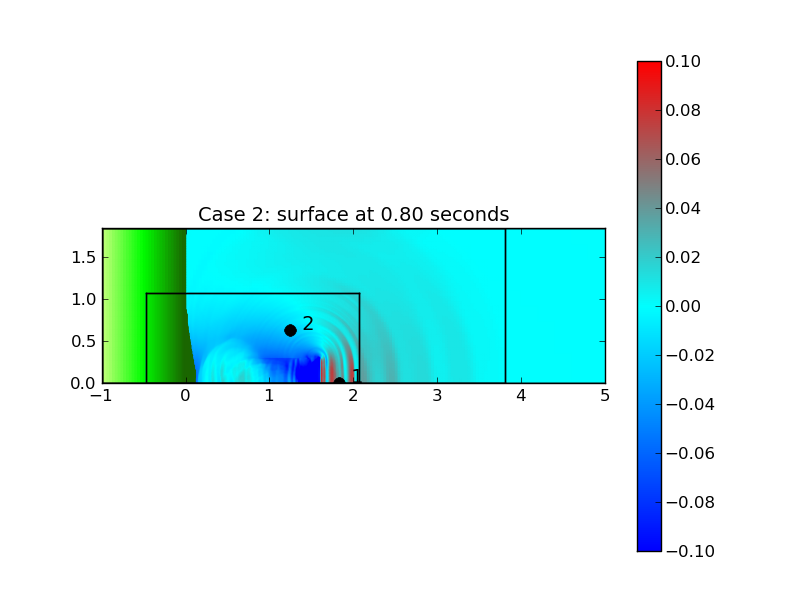
\includegraphics[width=2.8in]{bp12/case2pcolor8.png}\hfil
\hfil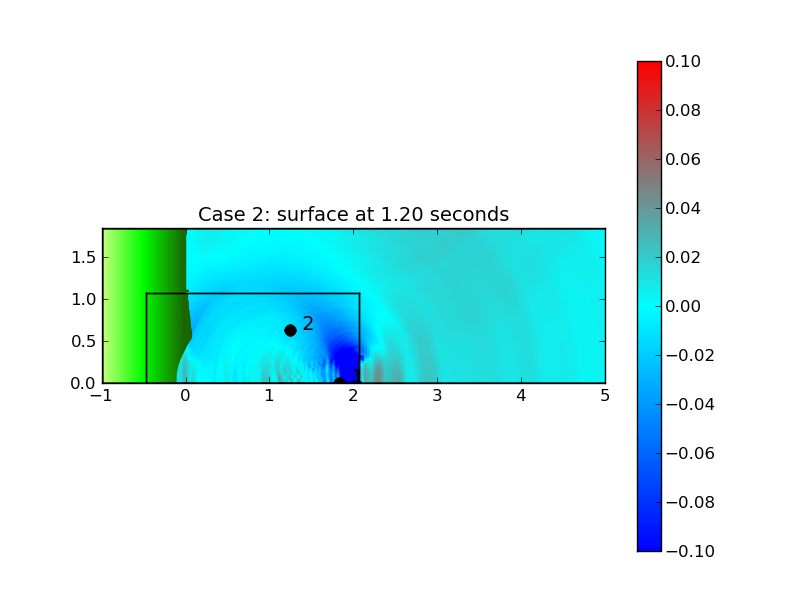
\includegraphics[width=2.8in]{bp12/case2pcolor12.png}\hfil
\caption{\label{fig:bp8pcolorcase2}
GeoClaw simulation for case 2 at times $t = 0,$ 0.4, 0.8, and 1.2.
  }
\end{figure}
}

\subsubsection{Gauge comparisons}

\Fig{bp8gauges1} shows a comparison of the GeoClaw results with the
laboratory values at the two wave gauges and two runup gauges requested
for case 1.  The gauge data for gauge 1 is initially very ``noisy" but the overall
behavior seems to be captured well.  We suspect that since gauge 1 was in
the wedge's path of travel and since the wedge was specified as part of our
bathymetry, this created heavy oscillations in our wave formations.  This can
best be observed by looking at \Fig{bp8pcolorcase1} for time 0.8 seconds.
The results are in general a good match to the laboratory measurements.

\begin{figure}[ht]
\hfil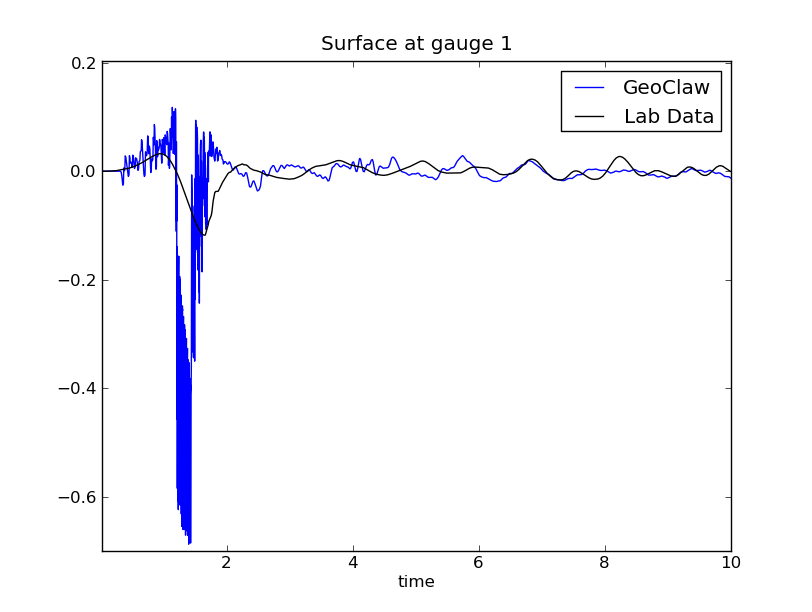
\includegraphics[width=2.8in]{bp12/case1wavegauge1.png}\hfil
\hfil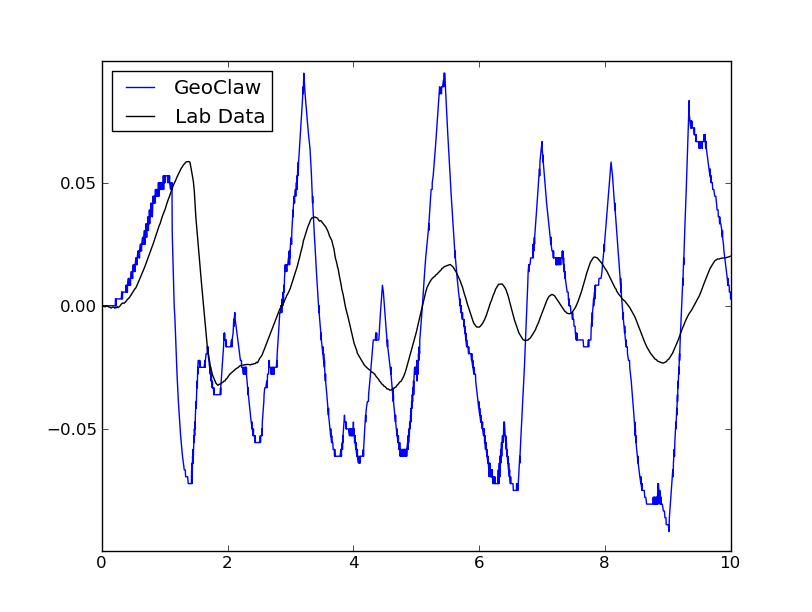
\includegraphics[width=2.8in]{bp12/case1runupgauge2.png}\hfil
\vskip 5pt
\hfil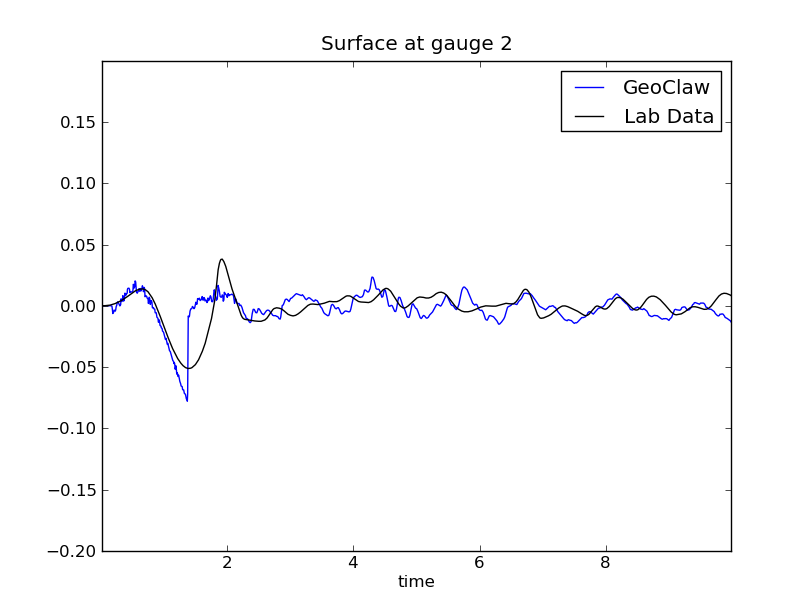
\includegraphics[width=2.8in]{bp12/case1wavegauge2.png}\hfil
\hfil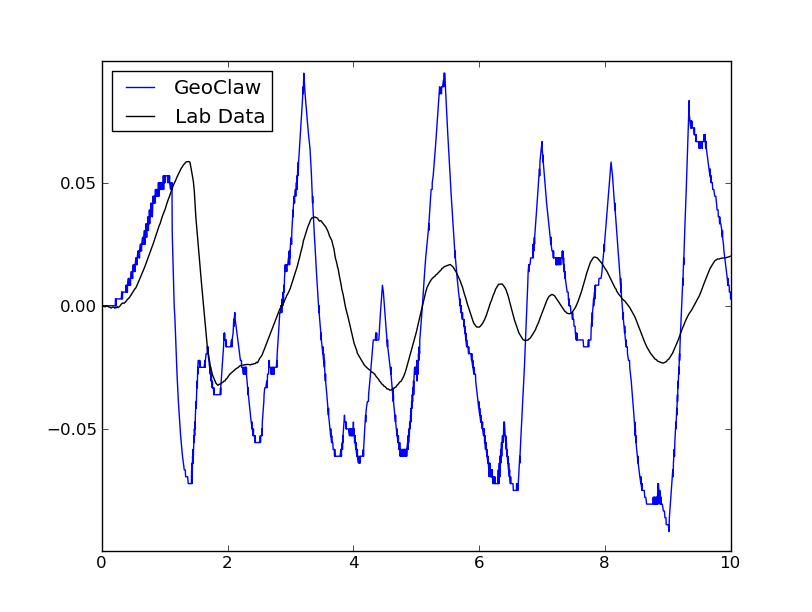
\includegraphics[width=2.8in]{bp12/case1runupgauge2.png}\hfil
\caption{\label{fig:bp8gauges1}
Left column: Time histories of the surface elevation with respect to still
water level for case 1.
Right column: Time histories of the runup measurements with respect
to still water level for case 1.
  }
\end{figure}



\Fig{bp8gauges2} shows a comparison of the GeoClaw results with the
laboratory values at the two wave gauges and two runup gauges requested
for case 2.  As was the case for case 1, the gauge data for gauge 1 is initially
very ``noisy" but the overall behavior seems to be captured well.  In looking at
\Fig{bp8pcolorcase2} for time 0.8 seconds, one can see why this seems to 
occur.  The results are in general a good match to the laboratory
measurements.

\begin{figure}[ht]
\hfil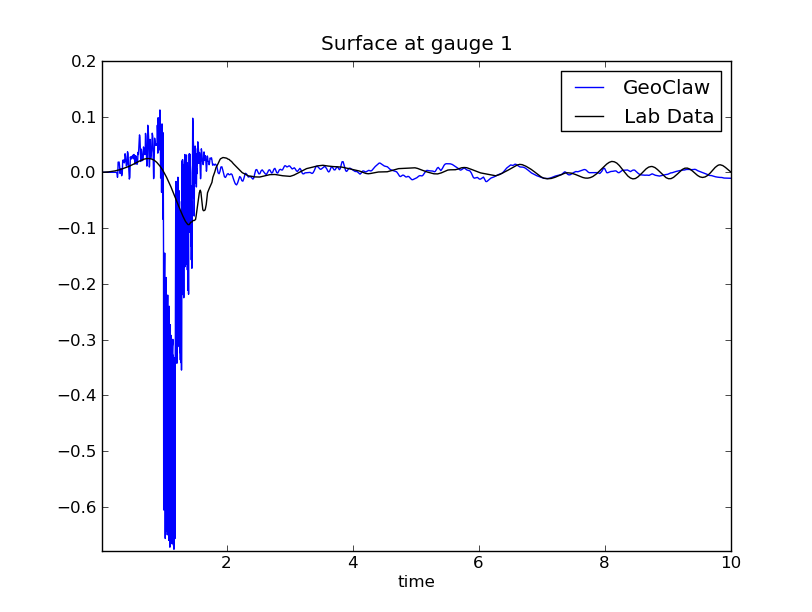
\includegraphics[width=2.8in]{bp12/case2wavegauge1.png}\hfil
\hfil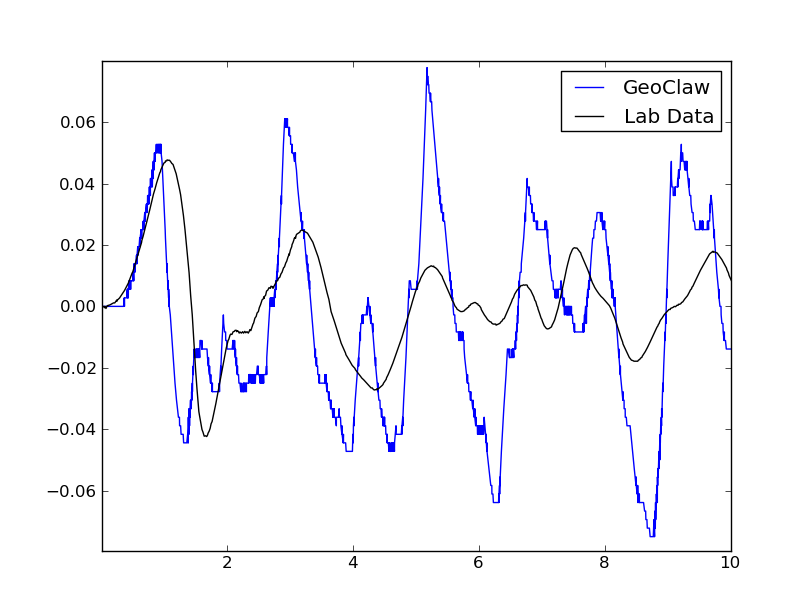
\includegraphics[width=2.8in]{bp12/case2runupgauge2.png}\hfil
\vskip 5pt
\hfil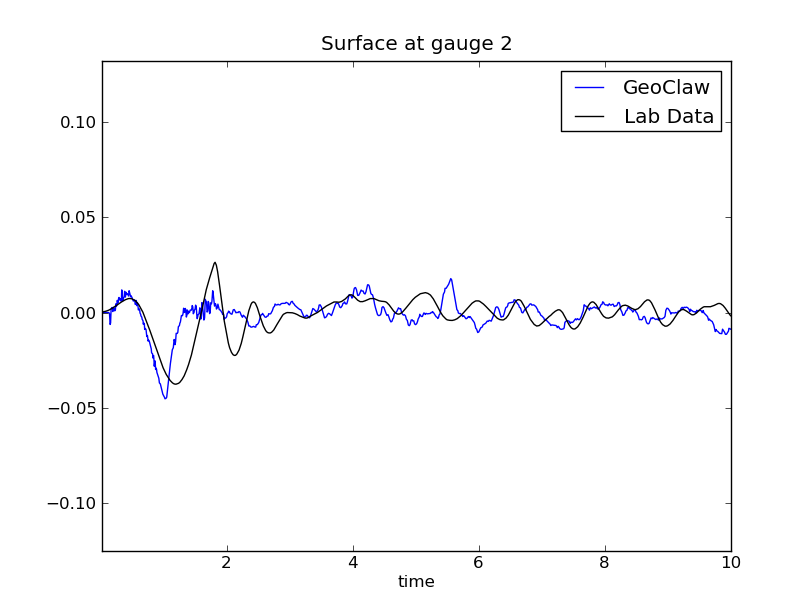
\includegraphics[width=2.8in]{bp12/case2wavegauge2.png}\hfil
\hfil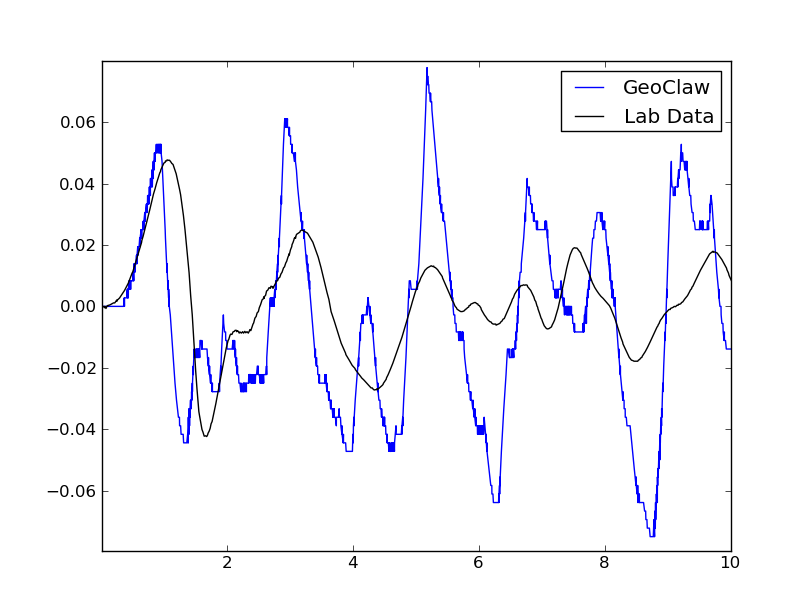
\includegraphics[width=2.8in]{bp12/case2runupgauge2.png}\hfil
\caption{\label{fig:bp8gauges2}
Left column: Time histories of the surface elevation with respect to still
water level for case 2.
Right column: Time histories of the runup measurements with respect
to still water level for case 2.
  }
\end{figure}


\subsubsection{Lessons learned}


\begin{itemize}
\item
It is not clear that the shallow water equations are a good model for this
problem.  The flow should be fully three-dimensional around this sliding
wedge and it is not clear that any depth-averaged model will do well.

\item At some distance away from the shore, 
the depth will be greater than wave length and the shallow water equations
will no longer be valid.

\item The vertical face causes numerical difficulties.

\item 
Overall, GeoClaw seems to model the surface elevations with respect to still water
level well for both cases.  However, gauge 1 seems to have issues from shortly
after the start of the simulation to about 2 seconds.  As mentioned earlier, it seems
that this phenomena is more of a result of how the bathymetry is specified than
GeoClaw's ability to model this landslide.  To smooth the data, one could try 
interpolating the data so that the moving bathymetry is smooth instead of
piecewise.  This should greatly reduce the heavy oscillations.  Another approach
would be to add a slope to the leading face of the wedge.  This would ensure a 
more gradual drop in bathymetry as the wedge propagates across the linear
beach.


\item
This benchmark problem does not appear to be a good test for tsunami models.
The dimensions do not seem to be reasonable relative to true submarine
landslides problems.  The vertical face does not seem realistic and causes
numerical difficulties.

\end{itemize} 
